\section{Programming}

\subsection*{6.1.1 and 6.1.2: Reusing Homework 1 and building the MLP}
The three \texttt{Copy from your HW1} blocks in \texttt{mlp.py} are adapted from my Homework 1 code to this skeleton's contract: \texttt{featurize} averages the GloVe vectors of the in-vocabulary tokens and returns \texttt{None} when there are none, \texttt{create\_tensor\_dataset} drops those reviews and stacks the rest into a float feature tensor and an \texttt{int64} label tensor, and \texttt{accuracy} takes the arg-max over the class dimension. The MLP builds one \texttt{nn.Linear} per consecutive pair in \texttt{[embed\_dim] + hidden\_dims + [num\_classes]}, so an empty \texttt{hidden\_dims} gives the single linear layer of Homework 1, and \texttt{forward} applies the activation after every layer except the last, because \texttt{CrossEntropyLoss} expects raw logits:
\begin{verbatim}
layer_dims = [embed_dim] + list(hidden_dims) + [num_classes]
for in_dim, out_dim in zip(layer_dims[:-1], layer_dims[1:]):
    self.linears.append(nn.Linear(in_dim, out_dim))
...
hidden = inp                                  # (batch_size, embed_dim)
for linear in self.linears[:-1]:
    hidden = self.activation(linear(hidden))  # (batch_size, hidden_dims[i])
logits = self.linears[-1](hidden)             # (batch_size, num_classes)
\end{verbatim}
Before training, the layer shapes were checked for all four configurations, \texttt{forward} was checked against a hand-written composition of the same layers, and \texttt{featurize} and \texttt{accuracy} were checked on small inputs.

\textbf{Setup shared by every run in Section 6.} IMDB, shuffled once with seed 42 (the skeleton's \texttt{shuffle()} was unseeded, and seeding it makes the split reproducible). Dev is the first 1{,}000 training reviews, train the next 20{,}000, and test the first 1{,}000 test reviews. Features are the average \texttt{glove-twitter-50} vector of the NLTK tokens of the lower-cased review. Training uses Adam and cross-entropy for 20 epochs, and the checkpoint with the best dev accuracy is scored on the test set. With 1{,}000 dev reviews, the standard error of an accuracy near 77\% is $\sqrt{0.77\cdot0.23/1000}\approx1.3$ points, which is the scale of the epoch-to-epoch wiggles in every plot below.

\subsection*{6.1.3 Train and evaluate MLPs}
Configurations from \texttt{explore\_mlp\_structures} (sigmoid activation, batch size 64). The template assigns each depth its own learning rate, so depth and step size change together in this experiment.

\begin{center}\small
\begin{tabular}{lccccc}
\toprule
Hidden layers & Learning rate & Dev acc.\ after epoch 0 & Best dev acc. & Min dev loss & Test acc.\\
\midrule
None (linear) & 0.025 & 0.744 & 0.771 & 0.481 & 0.770\\
512 & 0.02 & 0.743 & 0.779 & 0.472 & 0.767\\
512 $\to$ 512 & 0.01 & 0.709 & 0.777 & 0.471 & 0.774\\
512 $\to$ 512 $\to$ 512 & 0.001 & 0.686 & 0.767 & 0.480 & 0.778\\
\bottomrule
\end{tabular}
\end{center}

\begin{figure}[H]
\centering
\begin{subfigure}{0.48\textwidth}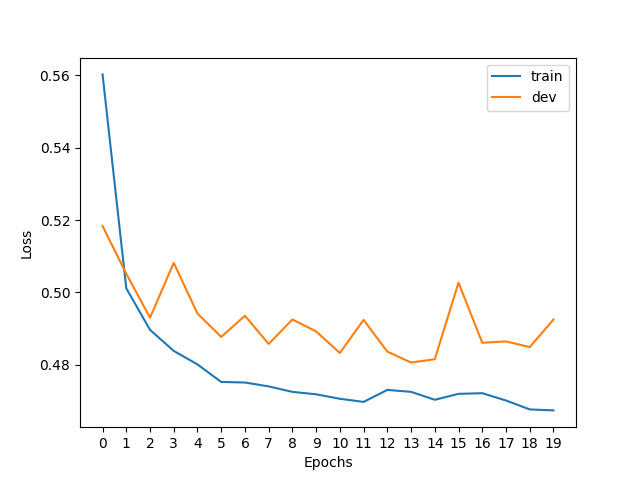
\includegraphics[width=\linewidth]{../hw3/mlp_None_loss.png}\caption{No hidden layer}\end{subfigure}\hfill
\begin{subfigure}{0.48\textwidth}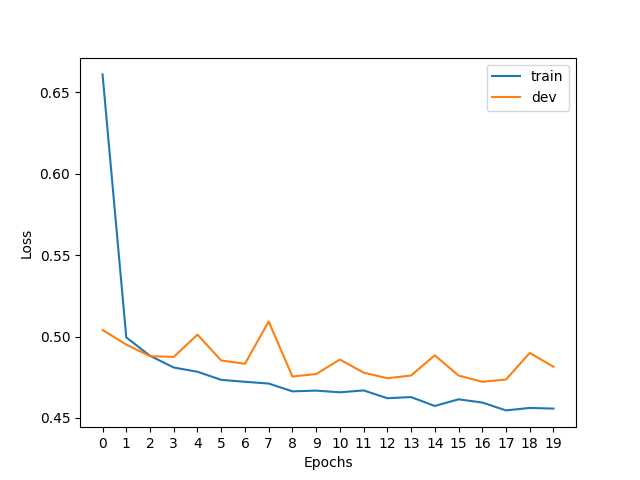
\includegraphics[width=\linewidth]{../hw3/mlp_512_loss.png}\caption{512}\end{subfigure}\\[4pt]
\begin{subfigure}{0.48\textwidth}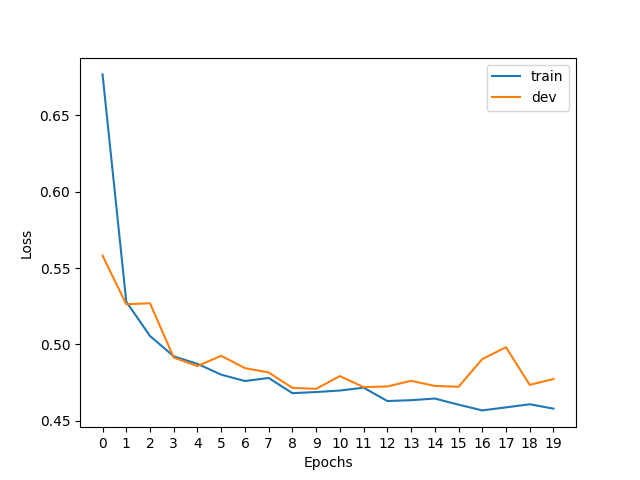
\includegraphics[width=\linewidth]{../hw3/mlp_512-512_loss.png}\caption{512 $\to$ 512}\end{subfigure}\hfill
\begin{subfigure}{0.48\textwidth}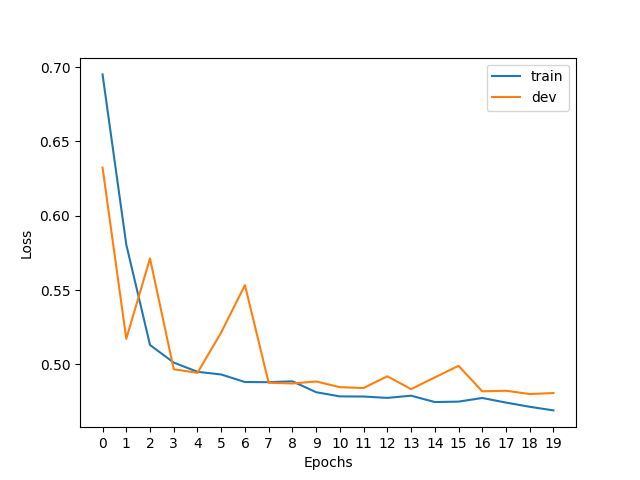
\includegraphics[width=\linewidth]{../hw3/mlp_512-512-512_loss.png}\caption{512 $\to$ 512 $\to$ 512}\end{subfigure}
\caption{Train and dev loss per epoch for each MLP configuration.}
\end{figure}

\begin{figure}[H]
\centering
\begin{subfigure}{0.48\textwidth}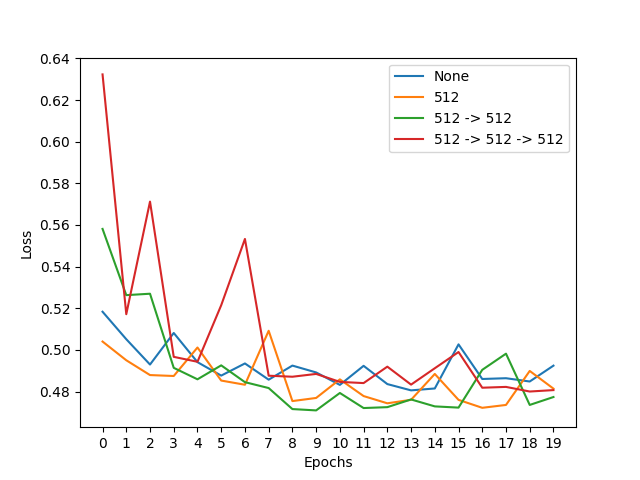
\includegraphics[width=\linewidth]{../hw3/all_mlp_loss.png}\caption{Dev loss}\end{subfigure}\hfill
\begin{subfigure}{0.48\textwidth}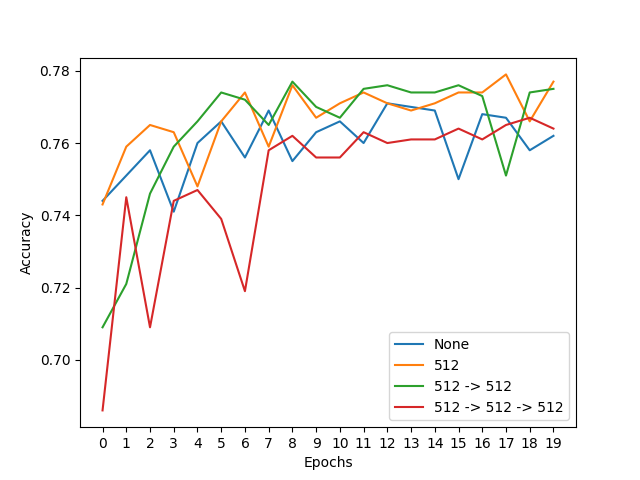
\includegraphics[width=\linewidth]{../hw3/all_mlp_acc.png}\caption{Dev accuracy}\end{subfigure}
\caption{Dev loss and dev accuracy across MLP configurations.}
\end{figure}

\textbf{Findings.} Train loss keeps falling in every configuration while dev loss levels off at 0.47 to 0.49, and the two deeper networks start lower (table) and have bumpier dev curves. Deeper is not better: best dev accuracy is 77.1\%, 77.9\%, 77.7\%, and 76.7\% for zero to three hidden layers, a spread smaller than the noise of a 1{,}000-review dev set. Depth and learning rate change together in this template, so the run cannot separate them, but a likely reason for the flat result is that averaged word vectors discard word order and negation, which leaves extra layers little more information to use.

\subsection*{6.1.4 Embrace non-linearity: the activation functions}
\texttt{SentimentClassifier} takes an \texttt{activation} argument that selects \texttt{nn.Sigmoid}, \texttt{nn.Tanh}, \texttt{nn.ReLU}, \texttt{nn.GELU}, or \texttt{nn.LeakyReLU}, and \texttt{explore\_mlp\_activations} trains one model per activation with everything else fixed (one 512-unit hidden layer, learning rate 0.02, batch size 128, 20 epochs). The Canvas version of the class template does not contain this function, so its fixed hyper-parameters are taken from the upstream JHU CS 601.471/671 hw3 skeleton that this assignment comes from.

\begin{center}\small
\begin{tabular}{lccccc}
\toprule
Activation & Epoch-0 train loss & Best dev accuracy & Min dev loss & Final dev loss & Test accuracy\\
\midrule
Sigmoid & 0.695 & 0.784 & 0.471 & 0.498 & 0.771\\
Tanh & 0.615 & 0.774 & 0.473 & 0.473 & 0.781\\
ReLU & 0.599 & 0.774 & 0.477 & 0.505 & 0.767\\
GELU & 0.602 & 0.787 & 0.472 & 0.519 & 0.760\\
LeakyReLU & 0.570 & 0.778 & 0.464 & 0.464 & 0.774\\
\bottomrule
\end{tabular}
\end{center}

\begin{figure}[H]
\centering
\begin{subfigure}{0.48\textwidth}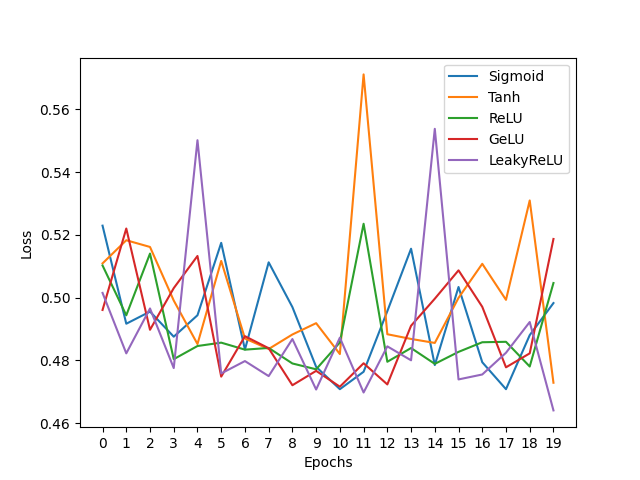
\includegraphics[width=\linewidth]{../hw3/all_mlp_activations_loss.png}\caption{Dev loss}\end{subfigure}\hfill
\begin{subfigure}{0.48\textwidth}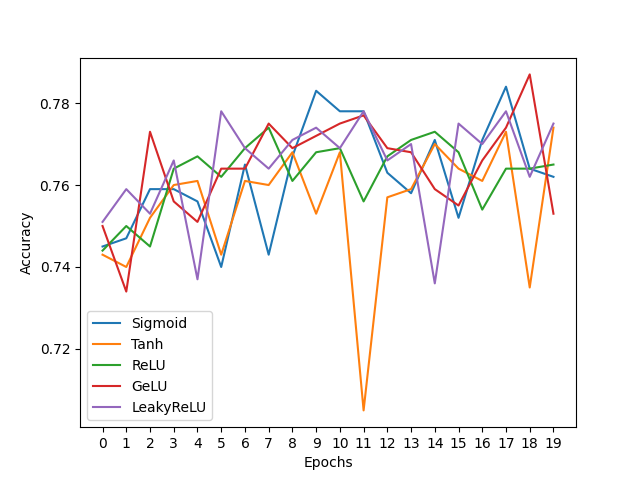
\includegraphics[width=\linewidth]{../hw3/all_mlp_activations_acc.png}\caption{Dev accuracy}\end{subfigure}
\caption{Dev loss and dev accuracy across activation functions (one 512-unit hidden layer).}
\end{figure}

\textbf{Findings.} All five activations end in the same place, with best dev accuracy between 77.4\% and 78.7\% and minimum dev loss between 0.464 and 0.477, differences inside the dev set's noise. Sigmoid starts slowest (average epoch-0 train loss 0.695, about $\ln 2$, against 0.57 to 0.62 for the others), consistent with its smaller slope ($\sigma'\le 1/4$) and its outputs not being zero-centered (Section 3.4), but all five reach 74\% to 75\% dev accuracy by the end of epoch 0. From epoch 5 on, each activation's dev loss moves within a band up to 0.10 wide (tanh), wider than any gap between activations, so keeping the best-dev checkpoint matters more than the choice of activation.

\subsection*{6.1.5 Hyper-parameter tuning: learning rate}
\texttt{explore\_mlp\_learning\_rates} trains the same single 512-unit sigmoid MLP (batch size 64, 20 epochs) at five learning rates: the provided 0.02 plus 0.1, 0.002, 0.0002, and 0.00002 (a factor of 5 above the default, then factors of 10 below it). A separate two-epoch check (\texttt{verification/}\allowbreak\texttt{check\_lr\_saturation.py}) counts how many hidden sigmoid outputs on the dev set are below 0.01 or above 0.99 at learning rates 0.1 and 0.02. It is a separate, seeded run, so its timing differs from the plotted one.

\begin{center}\small
\begin{tabular}{lcccc}
\toprule
Learning rate & Best dev accuracy & Min dev loss & Final dev loss & Test accuracy\\
\midrule
0.1 & 0.772 & 0.482 & 0.528 & 0.776\\
0.02 & 0.780 & 0.470 & 0.480 & 0.772\\
0.002 & 0.769 & 0.479 & 0.482 & 0.779\\
0.0002 & 0.750 & 0.499 & 0.499 & 0.739\\
0.00002 & 0.694 & 0.646 & 0.646 & 0.639\\
\bottomrule
\end{tabular}

\vspace{6pt}
\begin{tabular}{lccc}
\toprule
Saturation check & Epoch & Hidden sigmoid outputs saturated & Dev accuracy\\
\midrule
lr 0.1 & 0 & 100\% & 0.488\\
lr 0.1 & 1 & 99.8\% & 0.738\\
lr 0.02 & 0 & 0\% & 0.750\\
lr 0.02 & 1 & 0.6\% & 0.758\\
\bottomrule
\end{tabular}
\end{center}

\begin{figure}[H]
\centering
\begin{subfigure}{0.48\textwidth}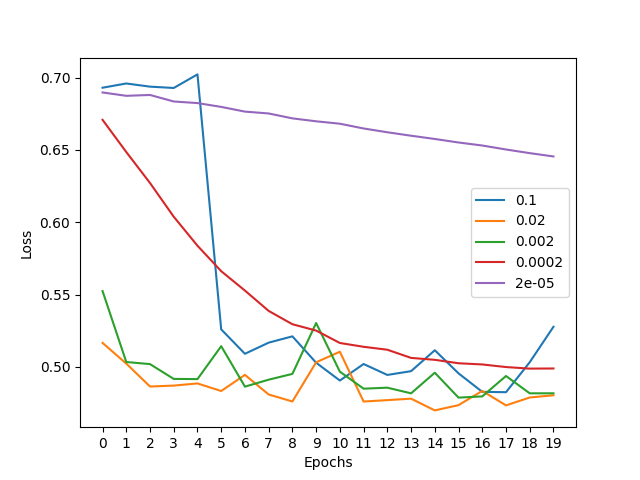
\includegraphics[width=\linewidth]{../hw3/all_mlp_lrs_loss.png}\caption{Dev loss}\end{subfigure}\hfill
\begin{subfigure}{0.48\textwidth}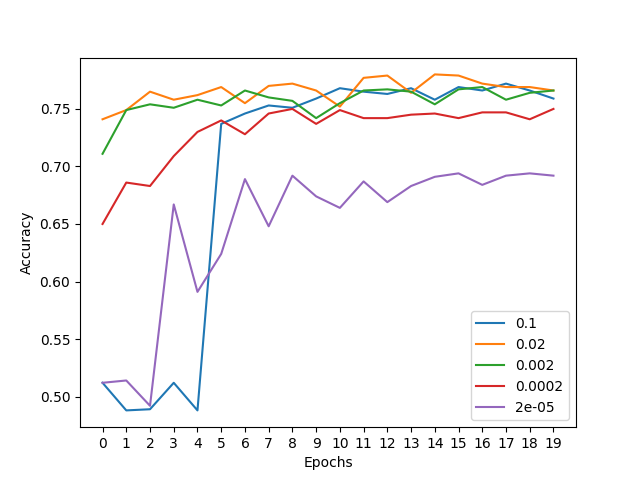
\includegraphics[width=\linewidth]{../hw3/all_mlp_lrs_acc.png}\caption{Dev accuracy}\end{subfigure}
\caption{Dev loss and dev accuracy across learning rates (one 512-unit sigmoid hidden layer).}
\end{figure}

\textbf{Findings.} Learning rates from 0.002 to 0.02 work about equally well (best dev accuracy 76.9\% and 78.0\%), and the provided 0.02 gets there fastest. At the extremes, 0.1 sits at chance for the first five epochs and still reaches 77.2\% at its best, while 0.0002 and 0.00002 improve smoothly but too slowly for 20 epochs and finish at 75.0\% and 69.2\%. The saturation check shows the large steps at 0.1 saturating every hidden sigmoid within one epoch, but accuracy recovered while they stayed saturated, so saturation explains the slow start only in part.
